\chapter{Ferramentas e ambiente de desenvolvimento}

No capítulo anterior, o VHDL foi apresentado como uma linguagem usada para descrever circuitos digitais. A partir deste ponto, além de entender a linguagem, é necessário preparar um ambiente de trabalho capaz de editar os arquivos, simular o comportamento do circuito e visualizar formas de onda. A implementação em FPGA será tratada mais adiante, quando os projetos já tiverem passado por simulações simples.

Este capítulo apresenta as ferramentas utilizadas no início da disciplina e propõe uma organização inicial para os arquivos dos projetos. A ideia não é transformar a instalação das ferramentas no objetivo principal, mas criar um fluxo simples e repetível para que cada exemplo da apostila possa ser editado, testado e documentado.

\begin{observacao}{Ideia-chave}
O ambiente de desenvolvimento deve ajudar o aluno a verificar o circuito antes de pensar na placa. A simulação nem sempre é uma etapa obrigatória em todos os projetos, mas é altamente recomendável para detectar erros antes da síntese. Por isso, nesta apostila, ela fará parte do fluxo de trabalho adotado.
\end{observacao}

\section{Visão geral do ambiente}

O fluxo adotado no início desta apostila combina ferramentas de edição, simulação e visualização. Outras ferramentas, como o Quartus Prime Lite, aparecem aqui apenas para situar o fluxo completo que será usado posteriormente. Cada ferramenta cumpre um papel diferente:

\begin{itemize}
    \item \textbf{Visual Studio Code:} editor utilizado para criar e organizar os arquivos VHDL.
    \item \textbf{VHDL for Professionals:} extensão do Visual Studio Code que auxilia na leitura, navegação e análise de arquivos VHDL.
    \item \textbf{GHDL:} ferramenta usada para analisar, elaborar e simular descrições VHDL.
    \item \textbf{VaporView:} visualizador de formas de onda geradas durante a simulação.
    \item \textbf{Quartus Prime Lite:} ferramenta da Intel que será usada mais adiante para sintetizar, implementar e gravar projetos em FPGAs compatíveis.
    \item \textbf{Tcl:} linguagem de scripts que poderá ser usada futuramente para automatizar comandos em ferramentas como o Quartus.
\end{itemize}

Essas ferramentas podem ser entendidas como partes de uma cadeia de trabalho. Primeiro, o projetista escreve os arquivos VHDL no editor. Em seguida, usa o GHDL para simular o circuito e gerar resultados. Quando a simulação produz uma forma de onda, o VaporView permite observar se as entradas e saídas se comportaram como esperado. A implementação em FPGA entra apenas depois dessa base estar bem estabelecida.

\begin{center}
\textbf{Edição} $\rightarrow$ \textbf{Simulação} $\rightarrow$ \textbf{Forma de onda} $\rightarrow$ \textbf{Síntese futura} $\rightarrow$ \textbf{FPGA}
\end{center}

\begin{observacao}{Antes de instalar tudo}
Nem toda ferramenta será usada com a mesma frequência no início da disciplina. Nos primeiros exemplos, o foco estará em editar arquivos VHDL, rodar simulações com GHDL e interpretar formas de onda. A instalação e o primeiro uso do Quartus serão tratados em um capítulo próprio, quando a apostila chegar à implementação em FPGA.
\end{observacao}

\section{Organização dos arquivos de projeto}

Antes de criar o primeiro projeto, é importante adotar uma estrutura de pastas simples. Isso evita confusão entre arquivos de código, arquivos de simulação, imagens, relatórios e saídas geradas automaticamente pelas ferramentas.

Uma organização recomendada para os exercícios da disciplina é:

\begin{lstlisting}[language={},caption={Estrutura sugerida para um projeto VHDL simples.},label={cod:estrutura-projeto}]
meu_projeto/
  src/
    porta_and.vhd
  sim/
    tb_porta_and.vhd
  waves/
    porta_and.vcd
  docs/
    anotacoes.md
\end{lstlisting}

Nessa estrutura, a pasta \texttt{src} guarda os arquivos VHDL que descrevem o circuito a ser sintetizado. A pasta \texttt{sim} guarda os \textit{testbenches} (bancadas de teste) e outros arquivos usados apenas para simulação. A pasta \texttt{waves} guarda arquivos de forma de onda, como \texttt{.vcd}. A pasta \texttt{docs} pode ser usada para anotações, tabelas de pinos, observações de teste ou pequenos relatórios.

Para projetos maiores, outras pastas podem ser adicionadas, como \texttt{constraints} para arquivos de restrições e \texttt{quartus} para arquivos específicos da ferramenta de síntese. No início, porém, uma estrutura pequena é suficiente e ajuda a reforçar uma separação importante: nem todo arquivo usado durante a simulação faz parte do circuito que será sintetizado.

\begin{observacao}{Síntese e simulação}
Arquivos de \textit{testbenches} normalmente não são sintetizáveis. Eles servem para estimular o circuito durante a simulação, mas não representam hardware que será gravado no FPGA. O próximo capítulo será dedicado a entender melhor o papel dos \textit{testbenches} e como eles se encaixam no fluxo de desenvolvimento.
\end{observacao}

\section{Instalação do Visual Studio Code}

O Visual Studio Code, também chamado de VS Code, é um editor de código desenvolvido pela Microsoft. Ele não é um simulador de VHDL e também não substitui ferramentas de síntese, como o Quartus. Seu papel neste fluxo é servir como ambiente de edição: nele serão criados, organizados e modificados os arquivos \texttt{.vhd}, \texttt{.vhdl}, scripts e demais arquivos do projeto.

A Figura~\ref{fig:vscode-logo} mostra o ícone oficial do Visual Studio Code. Ele pode ajudar a identificar o aplicativo correto durante a instalação, principalmente porque o nome é parecido com o do Visual Studio.

\begin{figure}[htbp]
    \centering
    
\includegraphics[width=0.16\textwidth]{figures/vscode-logo.png}
    \caption{Ícone oficial do Visual Studio Code.}
    \label{fig:vscode-logo}
\end{figure}

Para instalar o Visual Studio Code:

\begin{enumerate}
    \item Acesse a página oficial de download: \url{https://code.visualstudio.com/download}. A Figura~\ref{fig:vscode-download} mostra essa página.
    \item Na área correspondente ao seu sistema operacional, escolha o instalador adequado. No Windows, recomenda-se a opção \textit{User Installer} para a arquitetura do computador, normalmente \texttt{x64}.
    \item Após o download, execute o arquivo instalador.
    \item Avance pelas telas iniciais do assistente de instalação, aceitando os termos de uso quando solicitado.
    \item Na tela de tarefas adicionais, é recomendável marcar as opções para adicionar o VS Code ao menu de contexto e ao \texttt{PATH}, quando disponíveis. Isso facilita abrir pastas pelo terminal e usar comandos associados ao editor.
    \item Conclua a instalação e abra o Visual Studio Code.
\end{enumerate}

\begin{figure}[htbp]
    \centering
    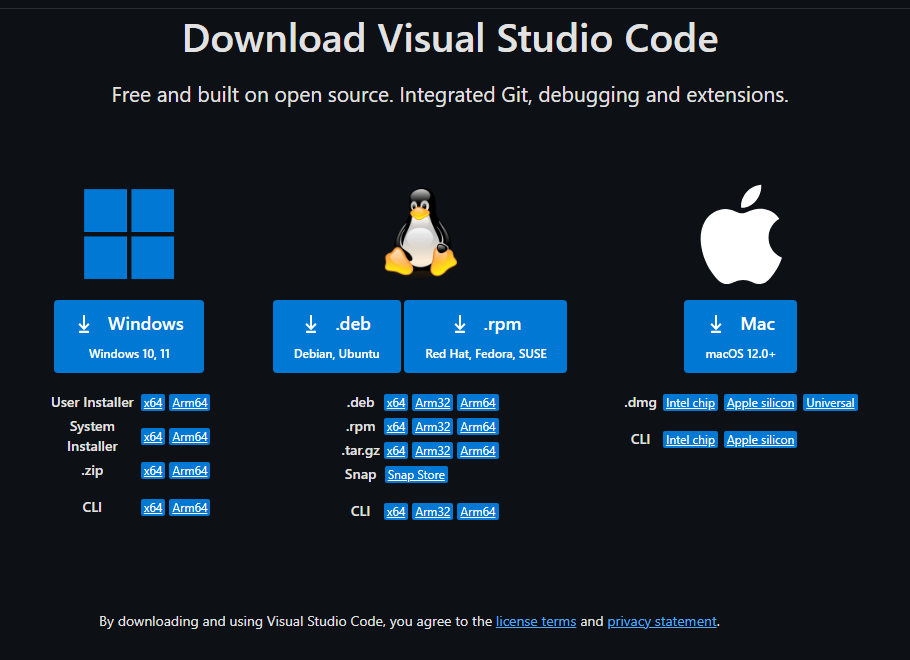
\includegraphics[width=0.95\textwidth]{figures/vscode-download-page.png}
    \caption{Página oficial de download do Visual Studio Code.}
    \label{fig:vscode-download}
\end{figure}

\begin{observacao}{Atenção ao nome}
Não confunda \textbf{Visual Studio Code} com \textbf{Visual Studio}. O Visual Studio é uma IDE maior, voltada principalmente para desenvolvimento de software em ambientes Microsoft. Nesta disciplina, será usado o Visual Studio Code.
\end{observacao}

Depois de abrir o VS Code pela primeira vez, observe a tela inicial e os menus principais. Diferente de outros editores, como o Notepad++, o VS Code trabalha em uma pasta de trabalho, ou seja, os arquivos são organizados dentro de uma pasta que representa o projeto. Para abrir uma pasta, use o menu \texttt{File > Open Folder} e selecione a pasta onde os arquivos do projeto serão criados.

Para abrir o terminal integrado, use o menu \texttt{Terminal > New Terminal}, ou pressione \texttt{Ctrl + `}. Neste momento, não é necessário executar comandos; a abertura do terminal serve apenas para localizar onde os comandos de simulação serão digitados futuramente.

A Figura~\ref{fig:vscode-interface} apresenta uma visão geral da interface do VS Code. Para os primeiros exercícios da disciplina, as regiões mais importantes são o explorador de arquivos à esquerda, o editor no centro e o painel inferior, onde o terminal integrado pode ser aberto.

As marcações da figura indicam as principais áreas do editor:

\begin{itemize}
    \item \textbf{Activity Bar:} barra lateral com ícones para alternar entre recursos do VS Code, como explorador de arquivos, busca, controle de versão, execução e extensões.
    \item \textbf{Primary Side Bar:} região lateral que mostra a ferramenta selecionada na \textit{Activity Bar}. No início da disciplina, ela será usada principalmente para visualizar a árvore de arquivos do projeto.
    \item \textbf{Editor Groups:} área central onde os arquivos são abertos e editados. É nessa região que os arquivos VHDL serão escritos.
    \item \textbf{Panel:} painel inferior usado para terminal integrado, mensagens de saída, problemas detectados e outras informações auxiliares. Quando a simulação com GHDL for introduzida, os comandos serão digitados nesse painel.
    \item \textbf{Status Bar:} barra inferior que mostra informações sobre o arquivo aberto e o ambiente, como linguagem reconhecida, codificação, quebras de linha e estado do projeto.
\end{itemize}

\begin{figure}[htbp]
    \centering
    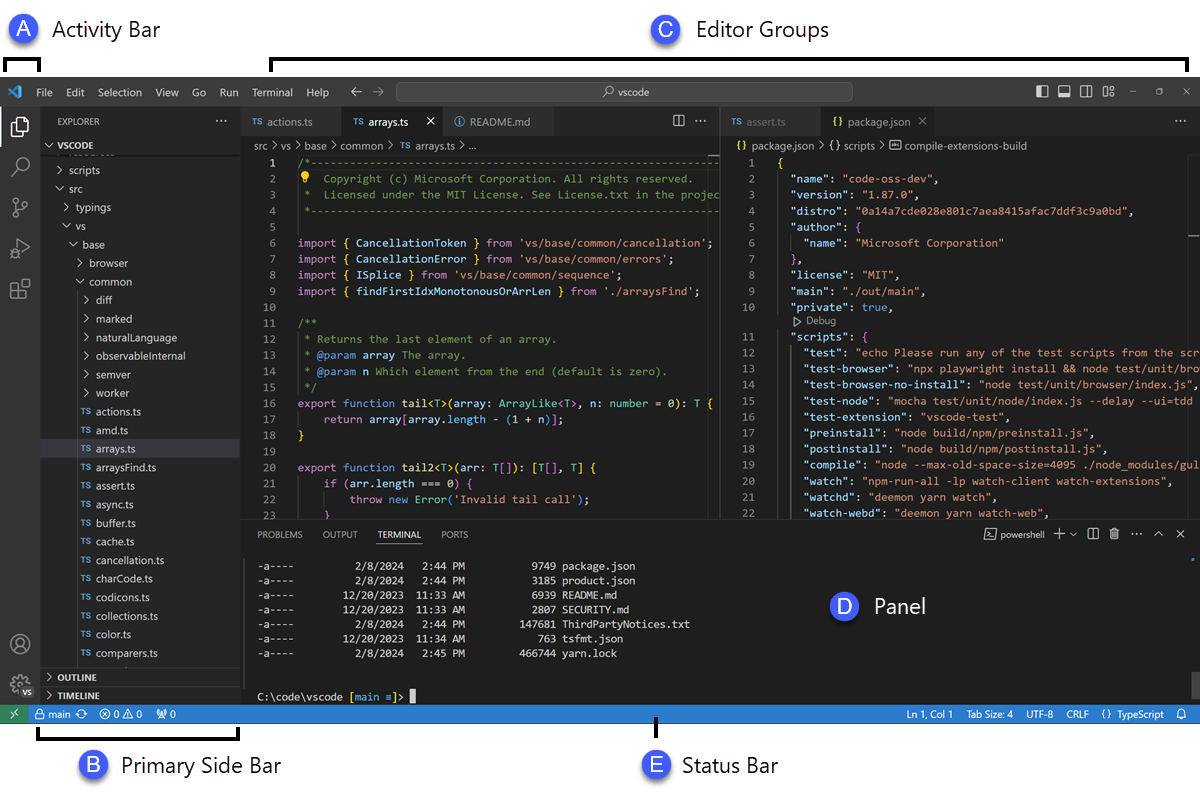
\includegraphics[width=\textwidth]{figures/vscode-user-interface.png}
    \caption{Interface do Visual Studio Code com as principais regiões do editor.}
    \label{fig:vscode-interface}
\end{figure}

\section{Configuração da extensão VHDL for Professionals}

A extensão VHDL for Professionals adiciona recursos de apoio à edição de arquivos VHDL no Visual Studio Code. Ela ajuda com destaque de sintaxe, navegação pelo código e algumas verificações durante a escrita. Isso torna o editor mais confortável, mas é importante separar os papéis: a extensão não substitui o GHDL, não executa simulações e não garante que o circuito esteja correto para síntese.

Para instalar a extensão, abra o Visual Studio Code e siga os passos abaixo:

\begin{enumerate}
    \item Na \textit{Activity Bar}, clique no ícone de extensões. Esse ícone é mostrado na Figura~\ref{fig:vscode-extensions-icon}. Outra forma de abrir a mesma área é usar o atalho \texttt{Ctrl+Shift+X}.
    \item Na caixa de busca da área de extensões, digite \texttt{VHDL for Professionals}.
    \item Localize a extensão chamada \textbf{VHDL for Professionals}. O publicador deve ser \texttt{ViDE-Software}. A Figura~\ref{fig:vhdl-professionals-marketplace} mostra a página da extensão no Marketplace do Visual Studio Code, com o nome, o publicador e o botão de instalação.
    \item Clique em \textit{Install} e aguarde a conclusão da instalação.
    \item Depois da instalação, abra um arquivo com extensão \texttt{.vhd} ou \texttt{.vhdl}. No canto inferior direito do VS Code, a \textit{Status Bar} deve indicar que a linguagem reconhecida é VHDL.
\end{enumerate}

\begin{figure}[htbp]
    \centering
    
\includegraphics[width=0.12\textwidth]{figures/vscode-extensions-icon.png}
    \caption{Ícone usado para abrir a área de extensões no Visual Studio Code.}
    \label{fig:vscode-extensions-icon}
\end{figure}

\begin{figure}[htbp]
    \centering
    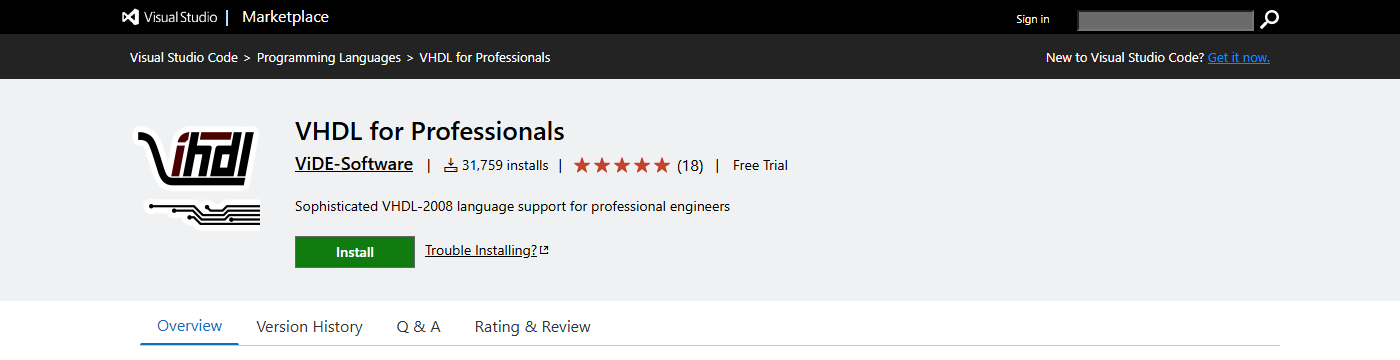
\includegraphics[width=\textwidth]{figures/vhdl-for-professionals-marketplace-crop.png}
    \caption{Página da extensão VHDL for Professionals no Marketplace do Visual Studio Code.}
    \label{fig:vhdl-professionals-marketplace}
\end{figure}

Se o VS Code não reconhecer automaticamente o arquivo como VHDL, clique no nome da linguagem exibido na \textit{Status Bar}, no canto inferior direito, e selecione \texttt{VHDL} manualmente. Essa verificação é simples, mas evita um problema comum: editar um arquivo VHDL como se fosse texto puro, sem destaque de sintaxe e sem os recursos da extensão.

A Figura~\ref{fig:vhdl-professionals-highlight} mostra um exemplo de apoio visual oferecido pela extensão durante a edição do código. Esse tipo de indicação ajuda a encontrar problemas enquanto o arquivo ainda está sendo escrito, antes mesmo de executar comandos de simulação.

\begin{figure}[htbp]
    \centering
    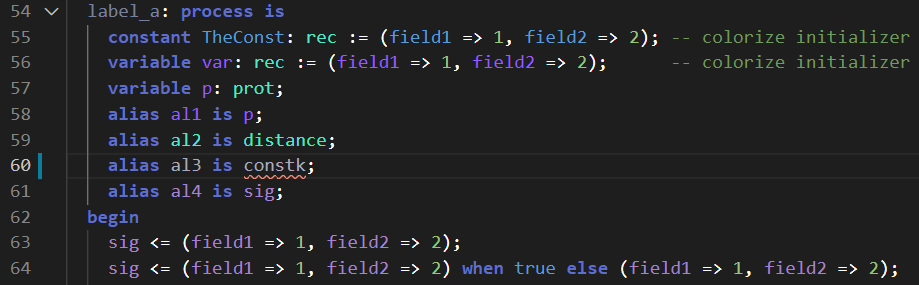
\includegraphics[width=0.92\textwidth]{figures/vhdl-for-professionals-highlight.png}
    \caption{Exemplo de destaque e indicação visual em código VHDL no editor.}
    \label{fig:vhdl-professionals-highlight}
\end{figure}

\section{Instalação do GHDL}

O GHDL é a ferramenta que será usada para analisar, elaborar e simular arquivos VHDL. Diferente da extensão instalada no Visual Studio Code, o GHDL não é apenas um recurso visual do editor: ele executa verificações sobre o código e permite observar o comportamento descrito antes de levar o projeto para uma ferramenta de síntese.

No Windows, a forma mais simples de instalar o GHDL é usando o \texttt{winget}, o gerenciador de pacotes do Windows. Antes de instalar, porém, é recomendável pesquisar o pacote disponível no próprio \texttt{winget}, pois o identificador do pacote pode mudar com o tempo.

Abra o terminal integrado do Visual Studio Code, ou o PowerShell do Windows, e execute:

\begin{lstlisting}[language={},caption={Pesquisa pelo pacote do GHDL no winget.},label={cod:winget-search-ghdl}]
winget search ghdl
\end{lstlisting}

Observe a lista exibida e procure uma entrada relacionada ao GHDL. No momento da escrita desta apostila, uma opção comum é o pacote identificado como \texttt{ghdl.ghdl.ucrt64.mcode}. Caso esse identificador apareça na busca, a instalação pode ser feita com:

\begin{lstlisting}[language={},caption={Instalação do GHDL pelo winget.},label={cod:winget-install-ghdl}]
winget install --id ghdl.ghdl.ucrt64.mcode --exact
\end{lstlisting}

Durante a instalação, o \texttt{winget} pode solicitar a aceitação dos termos da fonte de pacotes ou do instalador. Leia as mensagens exibidas no terminal e confirme quando apropriado. Ao final da instalação, feche e abra novamente o terminal para garantir que o caminho do GHDL seja reconhecido.

Para verificar se a instalação funcionou, execute:

\begin{lstlisting}[language={},caption={Verificação da instalação do GHDL.},label={cod:ghdl-version}]
ghdl --version
\end{lstlisting}

Se o comando exibir a versão do GHDL, a instalação está pronta para os próximos exemplos.

\begin{observacao}{Não pule a busca}
Mesmo que esta apostila mostre um identificador de pacote, execute primeiro \texttt{winget search ghdl}. Essa etapa confirma qual nome está disponível no computador no momento da instalação e evita depender de um identificador que pode ter sido alterado ou substituído no repositório do \texttt{winget}.
\end{observacao}

\section{Primeira simulação com GHDL}

\section{Instalação do VaporView}

\section{Visualização de formas de onda}

\section{O papel do Quartus no fluxo completo}

O Quartus Prime Lite será usado mais adiante na apostila, quando os circuitos simulados passarem a ser implementados fisicamente em uma placa FPGA. Neste capítulo, ele aparece apenas para situar o fluxo completo de desenvolvimento.

Enquanto o GHDL verifica o comportamento descrito em VHDL durante a simulação, o Quartus realiza etapas associadas ao hardware real: síntese lógica, implementação no dispositivo, análise temporal e geração do arquivo que será gravado no FPGA. Essas etapas exigem conhecimentos adicionais, como escolha do dispositivo, atribuição de pinos e interpretação de relatórios da ferramenta.

\begin{observacao}{Por que deixar o Quartus para depois?}
Instalar e configurar o Quartus antes de entender simulação pode deslocar o foco do aprendizado. Primeiro, a apostila constrói a base de descrição e verificação em VHDL. Depois, quando o circuito já puder ser validado no computador, o fluxo de implementação em FPGA será introduzido com mais contexto.
\end{observacao}

\section{Automação futura com Tcl}

\section{Fluxo de trabalho recomendado}

\section{Problemas comuns e verificação da instalação}

\section{Perguntas para revisão}
